\DontFrameThisInToc
\Annex{Annexe sur les assistants conversationnels (\textit{chatbots})}
\label{annex:B-ANNEXE-CHATBOTS}
	
	% INTRODUCTION DE L'ANNEXE.
	
	% Engoument pour les chatbots en 2019.
	Au début de ce doctorat (\texttt{octobre 2019}), nous pouvions noter que :
	\begin{itemize}
		\item selon \cite{costello-lodolce:2019:gartner-top-technologies}, \textguillemets{\textit{seuls $4$\% des clients de \texttt{Gartner} [déclaraient] utiliser des \textit{chatbots} sur leur lieu de travail, mais $40$\%} [avaient] \textit{l'intention de les mettre en oeuvre à court terme}} ;
		\item et selon \cite{goasduff:2019:chatbots-will-appeal}, \textguillemets{\textit{d'ici 2022, 70\% des employés} [interagiraient] \textit{quotidiennement avec les plateformes conversationnelles}}.
	\end{itemize}
	
	% Engoument pour les chatbots en 2023.
	Aujourd'hui (\texttt{octobre 2023}), le mot \textit{chatbot} est présent sur toutes les lèvres, surtout depuis la révolution des \texttt{IA} génératives lancées par \texttt{ChatGPT} (\cite{openai:2023:chatgpt}) :
	\begin{itemize}
		\item selon \cite{costello-lodolce:2022:gartner-predicts-chatbots}, une entreprise sur deux aurait actuellement recours à une forme de \textit{chatbot} pour gérer sa relation client, et \textguillemets{\textit{d'ici 2027, les \textit{chatbots} deviendront le principal canal de service client pour environ un quart des organisations}}.
	\end{itemize}

	% Annonce du plan.
	Dans cette annexe, nous allons détailler les points suivants :
	\begin{itemize}
		\item une présentation rapide de ce qu'est un assistant conversationnel et de ses principales utilisations (voir \textsc{Section~\ref{annex:B.1-ANNEXE-CHATBOTS-PRESENTATION}}) ;
		\item une description des approches principales permettent de concevoir un assistant conversationnel, avec leurs avantages et leurs inconvénients (voir \textsc{Section~\ref{annex:B.2-ANNEXE-CHATBOTS-APPROCHES}}) ;
		\item une discussion sur le dilemme des choix de conception (voir \textsc{Section~\ref{annex:B.3-ANNEXE-CHATBOTS-DILEMME}}).
	\end{itemize}
	
	% TABLE DES MATIÈRES DE L'ANNEXE.
	\minitoc
	
	% \texttt{Assistant Virtuel SNCF} (\cite{sncf:2018:agent-virtuel-sncf}) pour la réservation de billets de train ;
	% \texttt{Google Assistant} (\cite{google:2016:google-assistant-your}) et \texttt{Alexa} (\cite{alexa-internet:2018:keyword-research-competitor}) pour la gestion de la domotique.
	% \texttt{ELIZA} (\cite{weizenbaum:1966:eliza-computer-program}) pour simuler un entretien clinique en psychothérapie ;
	% \texttt{AI Dungeon} (\cite{latitude-inc.-oasis-tech-inc.:2019:ai-dungeon}) pour participer à la narration d'histoires interactives ;
	% \texttt{ChatGPT} (\cite{openai:2023:chatgpt}) et \texttt{BARD} (\cite{google:2023:bard-chat-based}) pour discuter avec des larges modèles de langues (\texttt{LLM}).

	%%%%%--------------------------------------------------------------------
	%%%%% Annexe B.1: Présentation rapide des assistants conversationnels
	%%%%%--------------------------------------------------------------------
	\newpage
	\section{Présentation rapide des assistants conversationnels}
	\label{annex:B.1-ANNEXE-CHATBOTS-PRESENTATION}
	
		%%% Fonctionnalités.
		Les \textit{chatbots} sont des robots conversationnels permettant à un utilisateur d'obtenir des informations ou d'automatiser des actions à l'aide d'instructions en langage naturel.
		\begin{itemize}
			\item[\faThumbsUp] L'utilisation de tels assistants comporte \textbf{plusieurs avantages} :
			ces derniers permettent de réduire les coûts en d'automatisant des tâches simples et répétitives (\textit{permettant aux ainsi aux humaines de se concentrer sur les autres tâches à risques ou à forte valeur ajoutée}),
			ils sont réactifs et toujours accessibles (\textit{au milieu de la nuit, les jours fériés, et même après 16h un vendredi après}),
			et ils ont un comportement stable quelle que soit la situation (\textit{pas de sauts d'humeur, de fatigue ou d'erreurs d'inattention}).
			\item[\faThumbsDown] Néanmoins, ces assistants rencontrent aussi \textbf{plusieurs inconvénients} :
			leur compréhension limitée du langage peut introduire des erreurs (\textit{lorsque le sujet est complexe, quand il y a trop ou trop peu de contexte}),
			ils manquent parfois de flexibilité ou d'empathie (\textit{nécessitant alors d'escalader la requête vers un opérateur humain}),
			et les tâches de conception ou de mises sous contrôle nécessitent des coûts importants (\textit{collecte et annotation de données, création de parcours de dialogue, vérification du comportement et des dérives, ...}).
		\end{itemize}
		
		
		%%% Applications.
		Ainsi, ces assistants sont utilisés dans de nombreux domaines :
		\begin{itemize}
			\item la \textbf{relation client à distance} (\textit{proposer une assistance 24/7, répondre aux questions fréquentes, automatiser la prise de rendez-vous, envoyer des formulaires de satisfaction, ...}) ;
			\item le \textbf{commerce en ligne} (\textit{remplir des formulaires de réservation ou de rétractation, suivre une commande, assurer le service après-vente, ...}) ;
			\item la \textbf{domotique} (\textit{gérer d'appareils connectés, écouter de la musique, interagir avec le \texttt{GPS}, être notifié en cas d'alerte intrusion, ...}) ;
			\item l'\textbf{accès à l'information} (\textit{consulter une base documentaire, favoriser l'éducation, vulgariser ou résumer des concepts, ...}) ; 
			\item le \textbf{divertissement} (\textit{raconter une histoire ou une blague, organiser un jeu narratif, organiser une sortie, simplement discuter lors d'une insomnie, ...}).
		\end{itemize}
		
		%%% Exemples.
		\begin{leftBarExamples}
			Parmi les exemples connus, nous avons :
			\begin{itemize}
				\item \texttt{Alexa} (\cite{alexa-internet:2018:keyword-research-competitor}) et \texttt{Google Assistant} (\cite{google:2016:google-assistant-your}), permettant de gérer des appareils connectés ;
				\item L'\texttt{Assistant Virtuel SNCF}, gérant l'achat de billets pour la SNCF (\cite{sncf:2018:agent-virtuel-sncf}) ;
				\item \texttt{Louis}, gérant le suivi des bagages d'Air France (\cite{air-france:2017:louis}) ;
				\item \texttt{AI Dungeon}, racontant des histoires interactives et des jeux de rôles (\cite{latitude-inc.-oasis-tech-inc.:2019:ai-dungeon}) ;
				\item \texttt{ChatGPT} (\cite{openai:2023:chatgpt}) ou \texttt{BARD} (\cite{google:2023:bard-chat-based}), permettant de discuter sur presque n'importe quel sujet...
				\item ...
			\end{itemize}
		\end{leftBarExamples}
	
		%%% Fonctionnalités

	%%%%%--------------------------------------------------------------------
	%%%%% Annexe B.2: Approches principales pour concevoir un \textit{chatbot}
	%%%%%--------------------------------------------------------------------
	\section{Approches de conception : \textit{task-oriented} vs \textit{chat-oriented}}
	\label{annex:B.2-ANNEXE-CHATBOTS-APPROCHES}
	
		%%% Introduction.
		Pour concevoir un assistant conversationnel, il faut \textbf{trois fonctionnalités} :
		\begin{enumerate}
			\item un moyen de \textit{comprendre la demande} et d'en extraire les informations importantes ;
			\item un moyen de \textit{gérer le dialogue} et de définir la prochaine action de l'assistant ;
			\item un moyen de \textit{répondre à l'utilisateur} ou de réaliser l'action demandée.
		\end{enumerate}
		
		
		%%% Classification \textit{task-oriented} vs \textit{chat-oriented}.
		Il existe de nombreuses façons d'agencer et d'implémenter de ces fonctionnalités, mais selon \cite{chen-etal:2017:survey-dialogue-systems}, nous pouvons les distinguer en \textbf{deux approches principales} en fonction de l'usage de l'assistant :
		\begin{enumerate}
			\item soit l'assistant est spécialisé pour une tâche bien déterminée (\textit{task-oriented}), dans ce cas sa conception se base traditionnellement sur une \textbf{approche symbolique} pour modéliser ses états de dialogue ;
			\item soit l'assistant est axé sur la fluidité de la conversation avec l'utilisateur (\textit{chat-oriented}), dans ce cas sa conception est plutôt basée sur une \textbf{approche numérique} (ou générative), utilisant un encodeur et un décodeur pour traiter la demande en un seul jet.
		\end{enumerate}
		
		% Figure illustrant ces deux approches.
		Ces deux approches bien connues sont illustrées dans la \textsc{Figure~\ref{figure:B.2-ANNEXE-CHATBOT-APPROCHES}} et seront détaillées dans les sections suivantes.
		%
		\begin{figure}[H]
			\centering
			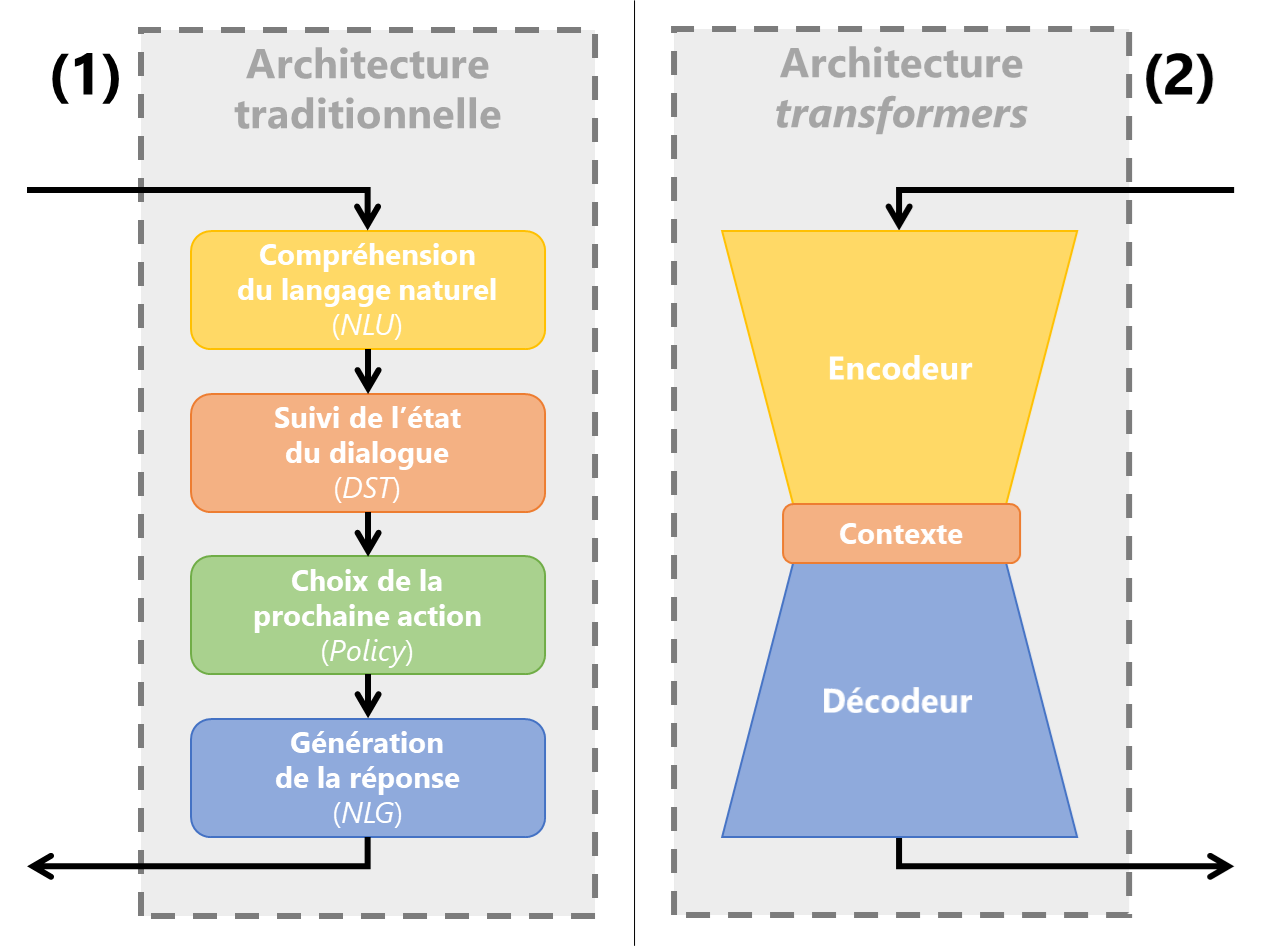
\includegraphics[width=0.90\textwidth]{figures/annexe-chatbots-architectures}
			\caption{
				Schéma illustrant les deux approches principales de conception d'un assistant conversationnel :
				\textbf{(1)} représente les \textbf{approches \textit{task-oriented}} à l'aide d'une architecture manipulant des états de dialogue ;
				\textbf{(2)} représente les \textbf{approches \textit{chat-oriented}} à l'aide d'une architecture à base de \textit{transformers}, encodant et décodant numériquement le dialogue et son contexte.
			}
			\label{figure:B.2-ANNEXE-CHATBOT-APPROCHES}
		\end{figure}
		
		%%%
		%%% Approches \textit{task-oriented}.
		

		%\cite{chen-etal:2017:survey-dialogue-systems}
		%\cite{adamopoulou-moussiades:2020:overview-chatbot-technology}.
		
			\todo[inline]{
				A REDIGER: \textit{task-oriented}\\
				Spécialisé tache \\
				Quelques exemples \\
				Architecture gestion d'état: NLP+DST+PL+NLG \\
				Contrôle du dialogue pour une tâche déterminée \\
				Peu de flexibilité
			}
			%%% DEFINITIONS:
			% Un \textit{chatbot} \textguillemets{\textit{task-oriented}} est conçu pour \textbf{accomplir une tâche spécifique}.
			% Le parcours de dialogue proposé est généralement prédéfini et comporte peu de digressions : l'assistant détermine l'action à réaliser grâce à l'énoncé de l'utilisateur, demande éventuellement des compléments d'informations si la requête n'est pas assez précise, puis effectue sa mission.
			% Le périmètre de fonctionnalités est généralement restreint pour contrôler les actions de l'assistant et s'assurer de son comportement.
			
			% ARCHITECTURE
			% \texttt{RASA} \cite{bocklisch-etal:2017:rasa-open-source}
			% \texttt{WATSON} (\cite{hoyt-etal:2016:ibm-watson-analytics}).
		
			%%% EXEMPLES:
			% \cite{schuurmans-frasincar:2020:intent-classification-dialogue} : definition intention
			% \cite{yan-etal:2017:building-taskoriented-dialogue} : projet task-oriented
			% \cite{brabra-etal:2022:dialogue-management-conversational}: plusieurs système de gestion du dialogue : soit implémenté manuellement, soit entraîné, soit hybride.
			
			%%% INSTRUCTIONS premières :
			% Pré-remplir d'un formulaire (\textit{réserver un billet de voyage, payer ses contraventions, faire opposition à sa carte de crédit, ...}) ;
			 % Gérer la domotique (\textit{allume la lumière, joue de la musique, active l'alarme, ...}).
			%%% INSTRUCTIONS secondaires :
			% Gérer la relation client (\textit{suivi de commande, formulaire de satisfaction, ...}) ;
			% Accéder à des informations documentaires ou personnelles (\textit{accès à une documentation technique, accès au solde d'un compte bancaire, ...}) ;
		
			%%% NOTES: une confusion fréquente est "task-based" => "not deep-learning"
			\begin{leftBarExamples}
				TODO
			\end{leftBarExamples}
		
		
		%%%
		%%% Approches \textit{chat-oriented}.
		%%%
		
			\todo[inline]{
				A REDIGER: \textit{chat-oriented}\\
				Axée dialogue \\
				Quelques exemples \\
				Architecture transformers: encodeur/décodeur, tout est numérique \\
				Pas de contrôle (hallucination) \\
				Grande flexibilité
			}
			%%% DEFINITIONS
			% Un \textit{chatbot} \textguillemets{\textit{chat-oriented}} se concentre davantage sur les interactions avec l'utilisateur dans le but d'\textbf{engager la conversation}.
			% Son objectif principale est de rendre le dialogue agréable.
			% Son périmètre de connaissance n'est en général pas restreint pour pouvoir facilement engager la conversation sur n'importe quel sujet.
			
			% ARCHITECTURE
			% \texttt{GPT} (\cite{openai:2023:chatgpt})
			% ou \texttt{LLAMA2} (\cite{touvron-etal:2023:llama-open-foundation}).
			% \cite{uszkoreit:2017:transformer-novel-neural}  \\ % architecture transformers
			% \cite{ni-etal:2022:recent-advances-deep}  \\ % avancer en deep learning
			% \cite{openai:2023:chatgpt}  \\ % exemple
			% \cite{touvron-etal:2023:llama-open-foundation}  \\ % exemple
			% \cite{kaddour-etal:2023:challenges-applications-large} % plusieurs challenges
			
			%%% FONCTIONNALITES
			% Offrir du divertissement (\textit{raconter une histoire ou une blague, organiser un jeu narratif, ...}) ;
			% Proposer une assistance générale (\textit{donner une définition, demander une explication, ...}) ;
			% Simplement discuter (\textit{mimer les interactions sociales}).
			
			\begin{leftBarExamples}
			\end{leftBarExamples}
		
		%%%
		%%% Approches hybrides.
		%%%
		
			\todo[inline]{
				A REDIGER: \textit{hybride}\\
				LLM instruct \\
				DST entraînée \\
				NLG décodeur
			}
			\begin{leftBarExamples}
				TODO
			\end{leftBarExamples}
	
	
	%%%%%--------------------------------------------------------------------
	%%%%% Annexe B.3: Dilemme de conception : entre flexibilité et contrôle.
	%%%%%--------------------------------------------------------------------
	\section{Dilemme de conception : entre flexibilité et contrôle}
	\label{annex:B.3-ANNEXE-CHATBOTS-DILEMME}
		
		\todo[inline]{A REDIGER: niveau d'automatisation}
		% \cite{sheridan-verplank:1978:human-computer-control} repris par \cite{parasuraman-etal:2000:model-types-levels} \\ % 10 niveaux de contrôles